
编译器优化对于高性能实现也很重要。运行一个编译时根本没有优化的程序,就能体会到编译器的作用,一个未优化的程序(优化级别为0)运行速度比启用所有优化后编译的程序慢一个数量级。

然而,优化器可以从开发者那里得到一些帮助。这种帮助可以通过非常微妙的形式,有时是反直觉的。在研究一些改进代码优化的技术之前,有助于理解编译器是如何处理程序的。

\subsubsubsection{10.2.1\hspace{0.2cm}编译器优化的基础知识}

关于优化必须了解的是,代码都必须保持正确。这里的正确与否与开发者主观认为什么是正确无关。程序可能会有错误,并给出一个看起来错误的答案,但编译器必须保留这个答案,而定义不明确或调用未定义行为的程序则是例外。如果程序在标准看来是错误的,编译器可以自由地做它想做的事情。我们将在下一章中来研究这一点。现在,我们将假设程序定义良好,并且只使用有效的C++语句。当然,由于答案不能因输入组合而改变,所以编译器在更改方面会受到限制。开发者可能知道某个输入值是正的,或者某个字符串中的字符永远不会超过16个,但编译器并不知道(除非找到一种方法来告诉它)。编译器只能够证明这种转换会产生完全等价的程序时,才能进行优化转换,从而该程序对任何输入都产生相同的输出。实际中,若是复杂性让编译器难以控制,编译器也会放弃修改。

理解这些是通过代码成功地与编译器交互,并实现更好的优化的关键。本章的其余部分展示了不同的方法,可以证明某些理想的优化并不会改变程序的行为。

编译器还受限于程序的信息。它只能处理编译时已知的内容,不了解任何运行时数据,并且假设运行时的合法状态都有可能。

下面是一个简单的例子:

\begin{lstlisting}[style=styleCXX]
std::vector<int> v;
… fill v with data … 
for (int& x : v) ++x;
\end{lstlisting}

关注的焦点是最后一行——循环。如果手动展开循环,性能可能会更好,每个增量都有一个分支(循环终止条件),展开循环可以减少此开销。在一个只有两个元素的简单\texttt{vector}例子中,最好完全删除循环,只对两个元素进行递增。但是,\texttt{vector}的大小是运行时的信息,编译器可能会生成一个带有一些分支的部分展开循环来处理所有可能的\texttt{vector}大小,但它无法针对特定大小对代码进行优化。

将它与下面的代码进行对比:

\begin{lstlisting}[style=styleCXX]
int v[16];
… fill v with data … 
for (int& x : v) ++x;
\end{lstlisting}

现在编译器确切地知道在循环中处理了多少整数,可以展开循环,甚至可以用一次操作多个数字的向量指令替换单个整数递增操作(例如,在x86上的AVX2指令可以一次处理8个整数)。 

如果开发者知道\texttt{vector}总是有16个元素呢?可能并不重要。重要的是编译器是否知道,并且能够确定无误,这比想象的要难。例如,以下代码:

\begin{lstlisting}[style=styleCXX]
constexpr size_t N = 16;
std::vector<int> v(N);
… fill v with data … 
for (int& x : v) ++x;
\end{lstlisting}

开发者用他们自己的方式使\texttt{vector}的大小成为一个编译时常量。编译器会优化循环吗?有可能。这完全取决于编译器能否确定\texttt{vector}的大小不会改变。它将如何改变?可以先问问自己,填充\texttt{vector}的代码中可能隐藏着什么?虽然对于开发者来说这是已知的,但如何让编译器也知道呢?所有的代码都是在构造和递增循环这两行之间编写的,编译器可以知道所有的东西(实际上,如果这个代码段太长,编译器就会放弃,并假设任何可能性,否则编译时间就会爆炸)。但若调用一个函数,而该函数可以访问\texttt{vector}对象,编译器则无法知道该函数是否改变了\texttt{vector}的大小(除非该函数是内联的)。像\texttt{fill\_vector\_without\_resizing()}这样的函数名,只对开发者阅读程序有帮助。 

即使没有函数以\texttt{v}作为参数,仍然不清楚函数要如何访问\texttt{vector}对象?如果\texttt{vector v}是在函数作用域中声明的局部变量,那可能不能。但如果\texttt{v}是一个全局变量,任何函数都可以访问它。类似地,如果\texttt{v}是类的成员变量,成员函数或友元函数都可以访问它。因此,如果调用一个非内联函数,这个函数不能通过参数直接访问\texttt{v},那么可以通过其他方式访问\texttt{v}(并且对于创建局部变量的全局指针这一邪恶的做法,知道的人越少越好)。 

从开发者的角度来看,很容易高估编译器所知道的东西。另外,在大多数情况下,把问题弄清楚并不是编译器的优点。例如:可以在循环之前添加一个断言:

\begin{lstlisting}[style=styleCXX]
constexpr size_t N = 16;
std::vector<int> v(N);
… fill v with data … 
assert(v.size() == N); // if (v.size() != N) abort();
for (int& x : v) ++x;
\end{lstlisting}

一些编译器在使用最高的优化级别和未优化的上下文中,会推断执行流不能进入循环,除非\texttt{vector}恰好有16个元素,并将优化该大小。并且,多数编译器不会这么做。

已经考虑过的基本示例中,用来帮助编译器优化代码的关键技术:

\begin{itemize}
\item
非内联函数会破坏大多数优化,因为编译器必须假设一个函数,但没有看到具体的代码,所以可以做任何合法的事情。 

\item
全局变量和共享变量对于优化有害。

\item
编译器更可能优化短而简单的代码,而不是长而复杂的代码。
	
\end{itemize}

第一个和最后一个在某种程度上有冲突。编译器中的大多数优化都局限于\textbf{基本代码块},这些块只有一个入口点和一个出口点,在程序的流控制图中充当节点。基本块之所以重要,是因为编译器可以看到块内发生的一切,因此可以对不改变输出的代码转换进行推理,所以内联的优点是它增加了基本块的大小。编译器不知道非内联函数在做什么,所以需要做最坏的假设。但若函数是内联的,编译器就能确切地知道它在做什么了(更重要的是,它没有做什么)。内联的缺点也在于它增加了基本块的大小,编译器只能分析这么多代码,而不会使编译时间变得不合理。内联对于编译器优化是非常重要的,原因我们将在后面进行讨论。

\subsubsubsection{10.2.2\hspace{0.2cm}函数内联}

当使用函数体的副本替换函数调用时,将由编译器执行。为了实现这一点,内联函数的定义必须在调用代码的编译过程中可见,调用的函数必须在编译时已知。第一个要求在进行全程序优化的编译器中是宽松的(不常见)。第二个要求排除虚函数调用和通过函数指针间接调用,并不是每个可以内联的函数最终都可以内联,编译器必须权衡代码膨胀和内联带来的好处。不同的编译器对于内联有不同的处理方法,C++的\texttt{inline}关键字只是一个建议,编译器可以忽视。

函数调用内联最明显的好处是消除了函数调用的成本。大多数情况下,当函数调用的开销不是那么大,也就不重要了。其主要的好处是,编译器跨函数调用的优化能力非常有限。考虑下面的代码:

\begin{lstlisting}[style=styleCXX]
double f(int& i, double x) {
	double res = g(x);
	++i;
	res += h(x);
	res += g(x);
	++i;
	res += h(x);
	return res;
}
\end{lstlisting}

以下是有效的优化吗?

\begin{lstlisting}[style=styleCXX]
double f(int& i, double x) {
	i += 2;
	return 2*(g(x) + h(x));
}
\end{lstlisting}

如果回答“是”,那么仍然是从开发者的角度,而不是从编译器的角度来看待这个问题。这种优化有很多方式会破坏代码(对于编写的合理的程序来说,可能没有一种是正确的,但编译器不能做的假设是自己是一个开发者)。 

\begin{itemize}
\item
首先,\texttt{g()}和\texttt{h()}可以产生输出。这种情况下,消除重复的函数调用将改变可观察行为。 

\item
其次,对\texttt{g()}的调用可能会锁定一些互斥对象,而对\texttt{h()}的调用可能会解锁它。这样,执行的顺序——调用\texttt{g()}锁定,增加\texttt{i}计数,调用\texttt{h()}解锁——就非常重要了。 

\item
第三,即使参数相同,\texttt{g()}和\texttt{h()}的结果也可能不同,例如:可以在内部使用随机数。 

\item
最后(这种可能性经常被忽略),变量\texttt{i}是通过引用传递的,所以不知道调用者还对它做了什么。可以是一个全局变量,或者某个对象可能会存储对它的引用,函数\texttt{g()}和\texttt{h()}可能会对\texttt{i}进行操作,即使没有看到它传入到这些函数中。 
	
\end{itemize}

另一方面,如果函数\texttt{g()}和\texttt{h()}内联,编译器可以确切地看到发生了什么:

\begin{lstlisting}[style=styleCXX]
double f(int& i, double x) {
	double res = x + 1; // g(x);
	++i;
	res += x – 1; // h(x);
	res += x + 1; // g(x)
	++i;
	res += x – 1; // h(x);
	return res;
}
\end{lstlisting}

整个函数\texttt{f()}现在是一个基本块,编译器只有一个限制:保留返回值。现在,就是一个有效的优化了:

\begin{lstlisting}[style=styleCXX]
double f(int& i, double x) {
	i += 2;
	return 4*x;
}
\end{lstlisting}

内联对优化的影响可以延伸到很远。考虑STL容器的析构函数,例如\texttt{std::vector<T>}。必须做的是调用容器中所有对象的析构函数:

\begin{lstlisting}[style=styleCXX]
for (auto it = crbegin(); it != crend(); ++it) it->~T();
\end{lstlisting}

因此,析构函数的执行时间与\texttt{vector}的大小N成正比。考虑一个由整数组成的\texttt{rstd::vector<int>},编译器非常清楚析构函数在这种情况下的作用:什么都不做。编译器还可以看到,对\texttt{crbegin()}和\texttt{crend()}的调用并不会修改\texttt{vector}对象(如果想通过\texttt{const\_iterator}销毁对象,请考虑如何销毁\texttt{const}对象)。因此,可以消除整个循环。

现在考虑使用结构体的\texttt{vector}:

\begin{lstlisting}[style=styleCXX]
struct S {
	long a;
	double x;
};
std::vector<S> v;
\end{lstlisting}

这一次,类型\texttt{T}有一个析构函数,并且编译器知道它的作用(因为通过编译器生成)。同样,析构函数什么也不做,整个销毁循环消除。对于默认析构函数也是如此:

\begin{lstlisting}[style=styleCXX]
struct S {
	long a;
	double x;
	~S() = default;
};
\end{lstlisting}

编译器应该能够为空析构函数做同样的优化,但只有内联时才会这么做:

\begin{lstlisting}[style=styleCXX]
struct S {
	long a;
	double x;
	~S() {}     // Probably optimized away
};
\end{lstlisting}

另一方面,如果类声明只是像下面这样声明析构函数:

\begin{lstlisting}[style=styleCXX]
struct S {
	long a;
	double x;
	~S();
};
\end{lstlisting}

定义是在单独的编译单元中提供的,然后编译器为每个\texttt{vector}元素生成一个函数调用。这个函数仍然什么也不做,但需要时间来运行循环,并执行N个函数调用。内联允许编译器将这优化为零。

这是内联及其对优化的影响的关键,内联允许编译器看到在本来神秘的函数中没有发生的事情。内联还有另一个重要的作用,创建内联函数体的唯一副本,可以使用调用者给出的特定输入进行优化。在这个唯一的副本中,可能会观察到一些对优化友好的条件,而这些条件对于函数通常是不正确的。下面是一个例子:

\begin{lstlisting}[style=styleCXX]
bool pred(int i) { return i == 0; }
… 
std::vector<int> v = … fill vector with data …;
auto it = std::find_if(v.begin(), v.end(), pred);
\end{lstlisting}

假设函数\texttt{pred()}的定义与对\texttt{std::find\_if()}的调用在同一个编译单元中,对\texttt{pred()}的调用是否内联?答案是“可能”,这主要取决于\texttt{find\_if()}是否内联。现在,\texttt{find\_if()}是模板,所以编译器可以看到函数的定义。如果\texttt{find\_if()}没有内联,则从模板中会为特定类型生成一个函数。这个函数中,第三个实参的类型是已知的:\texttt{bool (*)(int)}指向接受\texttt{int}类型并返回\texttt{bool}类型的函数的指针。但是这个指针在编译时未知,同一个\texttt{find\_if()}函数可以用许多不同的谓词来调用,这些谓词都不能是内联的。只有当编译器为这个特定的调用生成唯一的\texttt{find\_if()}副本时,谓词函数才能内联。编译器有时会这样做,这就是所谓的复制。但在大多数情况下,内联谓词或作为参数传入的其他内部函数的唯一方法,是首先内联外部函数。 

这个特殊的例子在不同的编译器上会产生不同的结果,GCC将只在最高的优化级别下内联\texttt{find\_if()}和\texttt{pred()}。其他编译器甚至不会这样做。然而,还有另一种方法鼓励编译器使用内联函数调用的方式,这似乎是反直觉的,因为这会向程序中添加了更多的代码,并使嵌套函数调用更加冗长:

\begin{lstlisting}[style=styleCXX]
bool pred(int i) { return i == 0; }
… 
std::vector<int> v = … fill vector with data …;
auto it = std::find_if(v.begin(), v.end(), 
  [&](int i) { return pred(i); });
\end{lstlisting}

这里的矛盾之处是,在同一个间接函数调用周围添加了一个间接层,即Lambda表达式(假设开发者不想简单地将谓词直接复制到Lambda中有其他的原因)。即使编译器没有内联\texttt{find\_if()},但\texttt{pred()}实际上更容易内联。因为,这一次谓词的类型是唯一的:每个Lambda表达式都有一个唯一的类型,因此对于这些特定的类型参数,\texttt{find\_if()}模板实例化一次。编译器可能会内联一个调用一次的函数,这样做就不会生成过多的代码。使对\texttt{find\_if()}的调用没有内联,但在该函数中,第三个参数只有一个可能,这个值在编译时就知道是\texttt{pred()}。因此,对\texttt{pred()}的调用可以内联。

现在,可以继续在第1章中提出的“虚函数调用的成本”问题了。首先,编译器使用函数指针表来实现虚调用,因此调用本身涉及到间接层。与非虚调用相比,CPU必须多读一个指针,并多做一次跳转。这为函数调用增加了更多的指令,使函数调用的代码开销增加了一倍(根据硬件和缓存状态有很大的变化)。然而,我们通常调用一个函数来完成工作,因此函数调用的机制只是函数执行总时间的一部分。即使对于简单函数,虚函数的开销也很少超过非虚函数的10-15\%。

然而,在花费太多时间计算指令之前,应该质疑最初的问题的有效性。如果一个非虚函数调用是充分的,也就在编译时就知道将调用哪个函数,为什么一开始要使用虚函数呢?如果发现只在运行时调用哪个函数,就根本不能使用非虚函数,因此它的速度无关紧要。按照这个逻辑,应该比较虚函数调用和函数等价的运行时解决方案,有条件地调用几个函数中的一个,使用一些运行时信息来选择。使用\texttt{if-else}或\texttt{switch}通常会导致执行速度变慢,至少在要调用函数有两个以上的重载版本时是这样。最有效的实现是使用函数指针表,这正是编译器对虚函数所做的。

当然,问题也并不是毫无意义。如果有一个带有虚函数的多态类,但是在某些情况下,在编译时就知道了实际的类型,该怎么办?这时,比较虚函数调用和非虚函数调用就有意义了。

还需要了解一下合适的编译器优化。如果编译器能够在编译时确定对象的真实类型,从而知道将调用虚拟函数的哪个重载版本,那么它将在去虚拟化中将调用转换为非虚的。

但是,为什么要在讨论内联的章节中讨论这个问题呢?因为我们忽略了一个事实,虚函数对性能的最大影响是(除非编译器可以反虚化调用)不能内联。一个简单的函数,如\texttt{int f() {return x;}}的结果是在内联之后只有一条,甚至没有指令,但是非内联版本具有常规的函数调用机制,就要慢一个数量级。若没有内联,编译器就无法知道虚函数内部发生了什么,必须对每一个外部可访问的数据块做出最坏的假设。所以在最坏的情况下,虚函数调用的代价可能会高出数千倍。

内联、展示函数体实现和创建唯一的、特化的函数副本的两种效果都有助于优化器,因为它们增加了编译器对代码的了解。若想帮助编译器更好地优化代码,那么理解编译器真正了解什么非常重要。 

现在,我们将探讨编译器在不同的约束下运行的情况,这样就可以发现错误的约束:一些是开发者认为是已知的,但编译器却不这么认为的情况。 

\subsubsubsection{10.2.3\hspace{0.2cm}编译器到底知道什么?}

也许对优化的最大限制是,了解在此代码执行期间可能会进行修改的内容。为什么这很重要?下面是一个例子:

\begin{lstlisting}[style=styleCXX]
int g(int a);
int f(const std::vector<int>& v, bool b) {
	int sum = 0;
	for (int a : v) {
		if (b) sum += g(a);
	}
	return sum;
} 
\end{lstlisting}

只有\texttt{g()}的声明是可用的。编译器能优化\texttt{if()}语句,并消除条件的重复求值吗?在经历了本章所有的惊喜和陷阱之后,我们可能正在寻找一个不这样做的原因。但结果是没有,这是一个完全有效的优化:

\begin{lstlisting}[style=styleCXX]
int f(const std::vector<int>& v, bool b) {
	if (!b) return 0;
	int sum = 0;
	for (int a : v) {
		sum += g(a);
	}
	return sum;
} 

\end{lstlisting}

现在让稍微修改一下这个例子:

\begin{lstlisting}[style=styleCXX]
int g(int a);
int f(const std::vector<int>& v, const bool& b) {
	int sum = 0;
	for (int a : v) {
		if (b) sum += g(a);
	}
	return sum;
} 
\end{lstlisting}

为什么要通过\texttt{const}引用传递\texttt{bool}形参呢?最常见的原因是模板。如果有一个模板函数不需要复制实参,则必须声明形参为\texttt{const T\&},这里假设\texttt{T}可以是任何类型。如果\texttt{T}推断为\texttt{bool}类型,那么现在就有了一个\texttt{const bool\&}形参。这里的变化可能很小,但对优化的影响是深远的。如果还认为之前所做的优化有效,请在更大的上下文中考虑我们的示例。现在可以看到所有内容(假设编译器仍然不可见):

\begin{lstlisting}[style=styleCXX]
bool flag = false;
int g(int a) {
	flag = a == 0;
	return –a;
}
int f(const std::vector<int>& v, const bool& b) {
	int sum = 0;
	for (int a : v) {
		if (b) sum += g(a);
	}
	return sum;
} 
int main() {
	f({0, 1, 2, 3, 4}, flag);
}
\end{lstlisting}

通过调用\texttt{g()},可以改变\texttt{b},因为\texttt{b}是一个绑定到全局变量的引用,该全局变量也可以在\texttt{g()}中访问。在第一次迭代中,\texttt{b}为false,但是对\texttt{g()}的调用有一个副作用,\texttt{b}变为了true。如果参数按值传递,则不会发生这种情况。值在函数最开始捕获,并且不跟踪调用者的变量。但是通过引用传递,并且循环的第二次迭代不再是固定的代码。每次迭代中,必须计算条件,并且不可能进行优化。再次强调,“开发者知道的”和“编译器知道的”之间的区别是,代码中没有全局变量,或者确切地知道函数\texttt{g()}的作用。编译器不能做出这样的猜测,并且必须假设程序做了(或在将来的某个时候会做)类似于前面的例子中演示的事情,这使得优化可能不安全。 

如果函数\texttt{g()}是内联的,并且编译器知道它没有修改全局变量,那么这种情况就不会发生。但不能期望所有代码都内联,因此在某些情况下,必须考虑如何帮助编译器确定它不知道的内容。当前的示例中,最简单的方法是引入一个临时变量(当然,在这个简单的示例中,可以手工进行优化,但这在更复杂的实际代码中并不实用)。为了让这个例子更真实一点,要记住函数\texttt{f()}可能来自一个模板的实例化。我们不想对未知类型的形参\texttt{b}进行复制,但知道它必须可以转换为\texttt{bool}类型,因此\texttt{bool}类型可以作为临时变量的类型:

\begin{lstlisting}[style=styleCXX]
template <typename T>
int f(const std::vector<int>& v, const T& t) {
	const bool b = bool(t);
	int sum = 0;
	for (int a: v) {
		if (b) sum += g(a);
	}
	return sum;
}
\end{lstlisting}

编译器仍然假设函数\texttt{g()}可能会改变\texttt{t}的值。但这不再重要,条件使用了临时变量\texttt{b},绝对不能改变,因为在函数\texttt{f()}之外不可见。当然,如果函数\texttt{g()}可以访问,并改变\texttt{f()}第二个参数的全局变量,那么转换就改变了程序的结果。通过创建这个临时变量,告诉编译器这种情况不会发生。这是编译器自己无法获得的信息。 

这很容易理解,但在实践中相当困难。若已知一些东西,但编译器不可能知道,就需要以一种编译器可以使用的方式进行断言。这很难做到的原因是,我们通常不会像编译器那样思考,而且很难放弃自己知道绝对正确的假设。 

这里把临时变量\texttt{b}声明为\texttt{const}了吗?这主要是为避免因意外修改而产生的错误,但这也有助于编译器。编译器能够看到没有改变\texttt{b}。与前面复杂的情况不同,编译器看到了对\texttt{b}的所有操作。然而,不能仅因为这些是可用的就确定编译器一定了解。分析程序需要时间,开发者只愿意等待编译器完成它的工作。另一方面,语法检查是必须的。如果声明变量\texttt{const}并试图修改,程序将无法编译,将不会进入优化步骤。因此,优化器可以假设\texttt{const}变量都不会改变。在可能的情况下将对象声明为\texttt{const}还有另一个原因,我们会在下一章中讨论这个问题。 

若已知一些东西,可以很尝试和编译器通信。这个建议确实违背了一个通用的建议:不要创建临时变量,除非它们使程序更容易阅读——编译器会删除它们。编译器可能确实会删除它们,但会保留(并使用)它们所表达的信息。

另一个阻止编译器进行优化的常见情况是混叠的可能性。下面是一个函数初始化两个C风格字符串的例子:

\begin{lstlisting}[style=styleCXX]
void init(char* a, char* b, size_t N) {
	for (size_t i = 0; i < N; ++i) {
		a[i] = '0';
		b[i] = '1';
	}
}

\end{lstlisting}

每次写入一个字节相当低效,有更好的方法来将所有字符初始化为相同的值。这个版本将会更快:

\hspace*{\fill} \\ %插入空行
\noindent
\textbf{08a\_restrict.C}
\begin{lstlisting}[style=styleCXX]
void init(char* a, char* b, size_t N) {
	std::memset(a, '0', N);
	std::memset(b, '1', N);
}
\end{lstlisting}

可以手工编写这段代码,但编译器不会做这种优化,理解其中的原因很重要。看到这个函数时,会希望它按照预期的方式使用,即初始化两个字符数组。但编译器必须考虑两个指针\texttt{a}和\texttt{b}是否指向同一个数组或者一个数组部分有重叠的可能性。以这种方式调用\texttt{init()}可能没有任何意义,这两个初始化将相互覆盖。然而,编译器只关心一个问题:如何不改变代码的行为。 

同样的问题也可能发生在通过引用或指针接受多个形参的函数中。例如以下函数:

\begin{lstlisting}[style=styleCXX]
void do_work(int& a, int& b, int& x) {
	if (x < 0) x = -x;
	a += x;
	b += x;
}
\end{lstlisting}

如果\texttt{a}、\texttt{b}和\texttt{x}绑定到同一个变量,编译器就不能做无效的优化。这就是所谓的别名:若同一个变量在代码中有两个不同的名字,则其中给一个名称即为别名。编译器必须在\texttt{a}递增后从内存中读取\texttt{x}。为什么呢?因为\texttt{a}和\texttt{x}可以指向相同的值,而编译器不能假设\texttt{x}保持不变。

如果确定不会发生混叠,该如何解决这个问题呢?C语言中,有一个关键字\texttt{restrict},它告诉编译器一个特定的指针是访问当前函数范围内的唯一方法:

\begin{lstlisting}[style=styleCXX]
void init(char* restrict a, char* restrict b, size_t N);
\end{lstlisting}

在\texttt{init()}函数中,编译器可以假设整个数组\texttt{a}只能通过这个指针访问,这也适用于标量变量。目前为止,\texttt{restrict}关键字还不是C++标准的一部分。即便如此,还是可以使用\texttt{restrict}, \texttt{\_\_restrict}、\texttt{\_\_restrict\_\_})表示,并且许多编译器还支持这个特性。对于奇异值(特别是引用),创建一个临时变量通常可以解决如下问题:

\hspace*{\fill} \\ %插入空行
\noindent
\textbf{09a\_restrict.C}
\begin{lstlisting}[style=styleCXX]
void do_work(int& a, int& b, int& x) {
	if (x < 0) x = -x;
	const int y = x;
	a += y;
	b += y;
}
\end{lstlisting}

编译器可能会消除临时变量(不为它分配任何内存),但现在它保证\texttt{a}和\texttt{b}都加了相同的数量。编译器真的会进行优化吗?最简单的方法是比较汇编输出,如下所示:

%\hspace*{\fill} \\ %插入空行
\begin{center}
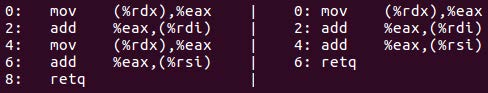
\includegraphics[width=0.9\textwidth]{content/3/chapter10/images/1.jpg}\\
图10.1 - x86汇编输出在优化之前(左)和之后(右)
\end{center}

图10.1展示了GCC为递增操作生成的x86汇编码(省略了函数调用和分支,两种情况下是相同的)。使用别名,编译器必须从内存中读取两次(mov指令)。在手动优化中,只有一次读取。

这些优化有多重要?其取决于许多因素,所以在没有进行一些测试之前,不应该着手一个消除代码中所有的别名。分析器会说明哪些部分是性能热点,那里有更多的优化机会。通过为编译器提供额外的信息,来帮助编译器的优化通常是最容易实现的(编译器已经做了最困难的工作)。 

向编译器提供有关程序的难以发现信息建议的另一方面是,不必担心编译器可以很容易地找到的东西。这个问题会在不同的上下文中出现,但更常见的场景是使用函数来验证输入。在库中,有一个用于交换指针的函数:

\begin{lstlisting}[style=styleCXX]
template <typename T>
void my_swap(T* p, T* q) {
	if (p && q) {
		using std::swap;
		swap(*p, *q);
	}
}
\end{lstlisting}

该函数接受空指针,但不对它们做任何操作。在代码中,由于某种原因,都必须检查指针,并且只有在两者都是非空的情况下才调用\texttt{my\_swap()}(如果它们是空的,也许需要做一些其他的事情,所以必须检查)。忽略其他工作,调用代码看起来会像这样:

\begin{lstlisting}[style=styleCXX]
void f(int* p, int* q) {
	if (p && q) my_swap(p, q);
}
\end{lstlisting}

C++开发者花费了过多的时间来争论冗余检查是否会影响性能。我们应该试着删除调用点的检查吗?假设不能,应该创建另一个版本的\texttt{my\_swap()},从而不测试它的输入吗?这里的关键是\texttt{my\_swap()}函数是一个模板(和一个小函数),所以肯定会内联。编译器拥有所有必要的信息来确定第二个null测试是冗余的。不是这样吗?比较两个程序的汇编输出,而不是尝试对可能的性能差异进行基准测试(在任何情况下,这个差异都是非常小的)。如果编译器生成的机器代码有冗余\texttt{if()}和没有冗余\texttt{if()},则可以确定没有性能差异。下面是GCC在x86上生成的汇编码:

%\hspace*{\fill} \\ %插入空行
\begin{center}
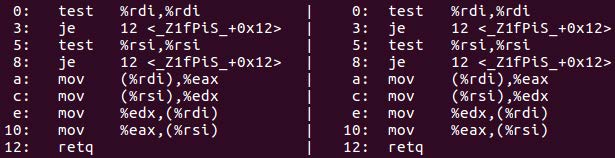
\includegraphics[width=0.9\textwidth]{content/3/chapter10/images/2.jpg}\\
图10.2 - 有(左)和没有(右)冗余指针测试的汇编码
\end{center}

图10.2的左边是为程序生成的两个\texttt{if()}语句的代码,一个在\texttt{my\_swap()}中,一个在外部。右边是\texttt{my\_swap()}的特殊非测试版本的程序代码。可以看到汇编代码是完全相同的(如果能够阅读x86汇编,还会注意到在这两种情况下只有两次比较,而不是四次)。 

内联在这里起着至关重要的作用。如果\texttt{my\_swap()}没有内联,在函数\texttt{f()}中进行第一次测试是不错的主意,因为避免了不必要的函数调用,并允许编译器可以更好地优化,以应对其中一个指针为空的情况。\texttt{my\_swap()}中的测试现在是冗余的,但编译器无会生成它,因为它不知道\texttt{my\_swap()}是否在别处调用,可能没有任何输入的保证。因为第二次测试是100\%可预测的(在第3章中讨论过),所以性能差异几乎没有。

这种情况最常见的可能是操作符\texttt{delete},C++允许删除空指针(什么都不会发生)。然而,许多开发者仍然这样写代码:

\begin{lstlisting}[style=styleCXX]
if (p) delete p; 
\end{lstlisting}

它是否会影响性能?不会。可以查看汇编输出,并说服自己,无论是否进行额外检查,都只对null进行了一次比较。 

现在,已经更好地理解了编译器如何阅读程序的。那么继续了解一种更有用的技术,它可以更好地进行编译器优化。

\subsubsubsection{10.2.4\hspace{0.2cm}将认知从运行时提升到编译时}

我们将在这里讨论的方法归结为,通过将运行时信息转换为编译时信息,为编译器提供有关程序的更多信息。下面的例子中,我们需要处理许多由\textit{Shape}类表示的几何对象。它们存储在一个容器中(如果类型是多态的,将是一个指针容器)。该处理包括两种操作之一:缩小或放大。让我们来看看代码:

\hspace*{\fill} \\ %插入空行
\noindent
\textbf{06\_template.C}
\begin{lstlisting}[style=styleCXX]
enum op_t { do_shrink, do_grow };
void process(std::vector<Shape>& v, op_t op) {
	for (Shape& s : v) {
		if (op == do_shrink) s.shrink();
		else s.grow();
	}
}
\end{lstlisting}

概括地说,有一个函数,它的行为在运行时由一个或多个变量控制。通常,这些变量都是布尔型(为了便于阅读,选择了枚举)。如果配置参数\texttt{op}通过引用传递,编译器必须将比较留在循环中,并对每个形状求值。即使参数是按值传递的,许多编译器也不会将分支提升出循环。需要复制循环体(一个循环用于收缩,一个循环用于增长),编译器担心代码过于膨胀。 

更大的可执行文件需要更长的加载时间,更多的代码增加了指令缓存的压力(i-cache,用于缓存即将到来的指令,就像数据缓存即将被CPU使用一样)。但在某些情况下,这种优化是正确的选择。通常,会在不更改配置变量的情况下处理大量数据。也许这些变量在整个程序运行过程中都是不变的(只加载一次配置,然后使用)。 

重写示例,将分支移出循环很容易,但如果代码很复杂,那么重构也会很复杂。如果愿意来帮助编译器,可以从编译器处得到一些帮助。其思想是将运行时值转换为编译时值:

\hspace*{\fill} \\ %插入空行
\noindent
\textbf{06\_template.C}
\begin{lstlisting}[style=styleCXX]
template <op_t op>
void process(std::vector<Shape>& v) {
	for (Shape& s : v) {
		if (op == do_shrink) s.shrink();
		else s.grow();
	}
}
void process(std::vector<Shape>& v, op_t op) {
	if (op == do_shrink) process<do_shrink>(v);
	else process<do_grow>(v);
}
\end{lstlisting}

整个(可能很大)旧函数\texttt{process()}转换为一个模板,除此之外,没有任何变化,没有将分支移出循环。但是,控制该分支的条件现在是一个编译时常量(模板参数),编译器会在每个模板实例化中消除分支和相应的固定代码。在程序的其余部分,配置变量仍然是一个运行时值,只是一个不经常更改(或根本不更改)的值罢了。因此,仍然需要一个运行时测试,但它仅用于决定调用哪个实例化的模板。

这种方法可以推广。假设需要计算每个形状的一些属性,比如体积、尺寸、重量等。这都可以由一个函数完成,因为许多计算可以在不同的属性之间共享。但需要时间来计算不需要的属性,所以可以实现这样的函数:

\begin{lstlisting}[style=styleCXX]
void measure(const std::vector<Shape>& s,
	double* length, double* width, double* depth,
	double* volume, double* weight);
\end{lstlisting}

空指针是有效的,表示不需要这个结果。在函数内部为请求值的特定组合编写最优的代码,只执行一次普通的计算。然而,这种检查是在循环中对形状进行的,这一次是一组相当复杂的条件。如果需要为同一组度量处理许多种形状,需要将条件提升到循环之外是有意义的,但编译器不太可能这样做(即使它可以)。同样,可以编写带有许多非类型形参的模板(它们将是布尔值),如\texttt{need\_length},\texttt{need\_width}等。在该模板内部,因为现在这是编译时信息,编译器将消除所有从未执行的分支。在运行时调用的函数必须根据指针是否为空,将数据调用或转发到正确的模板实例化。最有效的实现方式是查找表:

\hspace*{\fill} \\ %插入空行
\noindent
\textbf{07\_measure.C}
\begin{lstlisting}[style=styleCXX]
template <bool use_length, bool use_width, …>
void measure(const std::vector<Shape>& v,
double* length, … );
void measure(const std::vector<Shape>& v,
double* length, … ) {
	const int key = ((length != nullptr) << 0) |
					((width  != nullptr) << 1) |
				    ((depth  != nullptr) << 2) |
				    ((volume != nullptr) << 3) |
				    ((weight != nullptr) << 4);
	switch (key) {
		case 0x01: measure<true , false, … >(v, length, … );
		break;
		case 0x02: measure<false, true , … >(v, length, … );
		break;
		…
		default:; // Programming error, assert
	}
}
\end{lstlisting}

这将生成大量代码,测试的每个变体都是一个新函数。这样转换的效果应该通过分析来验证,但在测试相对简单的情况下(例如,许多形状都是一个立方体),并且对许多(数百万)形状请求相同的测试集时,这种修改可以获得更可观的性能收益。 

使用特定的编译器时,了解编译器的功能(包括优化)很有用。这样的详细程度超出了本书的范围,而且这是一种易变的知识——编译器发展得很快。相反,本章为理解编译器优化奠定了基础,并为读者提供了参考框架。


